\chapter{Simulation}
The activities of the simulation is described in this chapter.
An overview of NS-3 is given, which is then followed by the actions taken, setup
used, assumptions made and overall explanation of the simulation.

\section{NS-3}
A discrete event network simulator, NS-3 is used extensively in network research
and education. The workings and performance of packet data network are modelled
and NS-3 provides a platform for the simulation and experimentation of various
packet-based research. C++ and Python are the predominant language in which NS-3
is written with \textit{waf} as the build system. Design of NS-3 capitalizes on
the object oriented nature of these languages\cite{nsonline}.\\\\
There are various components of packet-based network, fundamentally there are the
endpoint devices, routers,NIC devices ,switches and the medium of exchange.
These components,however in NS-3, are abstracted to reflect what the components
actually do. The endpoint devices are called \textit{Nodes}, exchange medium
- \textit{Channel} and the applications that are generating the packets are 
\textit{Applications} just to name a few. The file/folder structure of a simulation
consist of a model which depicts the fine details of the simulation, a helper that
is supposed to include files containing the installation helper functions, an 
example folder to implement an example of the simulation. There are also doc and 
tests folders and the just as their names suggest they hold documentation and tests
files.\\\\
Installation of the NS-3 is not needed to get a simulation running, as the examples 
or experiments can be run using the binary files gotten from the build process.
It is actually not recommended to do installation of NS-3. Installation in this case
refers to running the command \textbf{\textit{./waf install}}.

\section{Setup}
The simulation was performed on a Gentoo Linux flavor computer with a 64 bit Intel
Eight-Core processor with model name \textit{Intel(R) Core(TM) i7-8565U CPU @
1.80GHz} and RAM of 32GB. Version 3-30 of NS-3 provided the platform on which to
undertake the research. At the time of setting up, this version was the latest most
stable release.\\\\
NS-3 is a voluminous software, the faster processor is needed, as a change to any
file would mean rebuilding the file and its dependencies and those that depend on it.
The version is also critical. Most versions are not backward compartible hence what
works on 3.29 might not work on 3.30 without a little tinkering.\\\\
Gentoo Linux, even though time consuming and quite advance in installation and
setting up, turns to be one of the fastest linux operating systems available. This is
partly due to the fact that source codes are compiled on the host computer with 
specific flags set for optimality.

\section{Components}
For a data packet to move from one endpoint to another, there are components such as,
the packet generating and receiving nodes which will have NIC, the medium(s) through
which the packet traverses also forms a part of the components.\\\\
There are three critical parts, worth mentioning for this simulation; the header which
is attached to the packet, tag-augmented sensor devices and the reader, which, in this
case, is augmented with a server.\\\\
A discussion of the various components follow next.
\subsection{Packet Header}
Various parts of a packet header which is added to a payload enable the packet to get
to its intended destination. A 4-byte(32 bits) header was created, having two fields
of 16 bits each representing the packet type being sent: data packet or broadcast 
and the state of the tag augmented sensor: whether a new data is available for 
transmission or not.\\
\begin{figure}[h!]
\begin{tikzpicture}
    \tikzumlset{font=\tiny\ttfamily}
    \umlemptyclass[x=0,y=0]{Header}{
}{}
\umlclass[x=5.5,y=-2]{AptMacHeader}{
  -m\_id : uint16\_t \\ -m\_type : uint16\_t \\ -m\_stateChange : uint16\_t
}{
  +AptMacHeader() \\ +SetId(id : uint16\_t) : void \\ +GetId (void) : const
  uint16\_t\\ +SetPacketType(ptype : uint16\_t) : void \\ +GetPacketType(void) :
  const uint16\_t \\ +SetStateChange(stateChange : uint16\_t) : void \\ 
  +GetStateChange(void) : const uint16\_t \\ \umlstatic{+GetTypeId(void) : TypeId}\\
  \umlvirt{+Serialize(start : Buffer::Iterator) : const void} \\
  \umlvirt{+Deserialize(start : Buffer::Iterator) : uint32\_t} \\
  \umlvirt{+GetSerializedSize(void) : const uint32\_t} \\
  \umlvirt{+GetInstanceTypeId (void) : const TypeId} \\
  \umlvirt{+Print(\&os : std::ostream) : const void}\\
}
\umlenum[x=11.5,y=-4]{HeaderContents}{
    BROADCAST : uint16\_t \\ DATA : uint16\_t \\ STATECHANGE : uint16\_t
}

%\umlassoc[geometry=-|-, arg1=tata, mult1=*, pos1=0.3, arg2=toto, mult2=1, pos2=2.9, align2=left]{C}{Header}
%\umlunicompo[geometry=-|, arg=titi, mult=*, pos=1.7, stereo=vector]{D}{C}
%\umlimport[geometry=|-, anchors=90 and 50, name=import]{sp2}{sp1}
\umlaggreg[geometry=-|]{AptMacHeader}{HeaderContents}
\umlinherit[geometry=-|]{AptMacHeader}{Header}
%\umlnote[x=2.5,y=-6, width=3cm]{B}{Je suis une note qui concerne la classe B}
%\umlnote[x=7.5,y=-2]{import-2}{Je suis une note qui concerne la relation d'import}
\end{tikzpicture}
\caption{Class Diagram - APT-MAC Header}
\label{fig:headerUML}
\end{figure}\\
The UML class diagram is illustrated in Figure \ref{fig:headerUML}. The \emph{
constructor, getter and setter} functions are for their usual purposes. \emph{
Serialize} function puts the various fields of the header in series by writing them
from host-order to network-order and the \emph{Deserialize} reads from network-order
to host-order. \emph{Enum HeaderContents} holds the value of the various fields of
the header.

\subsection{Tag Augmented Sensor Devices}
Devices in a smart home are broadly classified under three categories: periodic
(e.g., temperature sensors), real-time (e.g., joystick, cameras) and event based 
(e.g., presence detector, remote of appliances)\cite{Maselli}. The state changes
of the various devices were modelled according to Markov Chains\cite{Tolver}.\\
\begin{centering}
\begin{figure}[h!]
    \begin{subfigure}[b]{.5\textwidth}
        \centering
        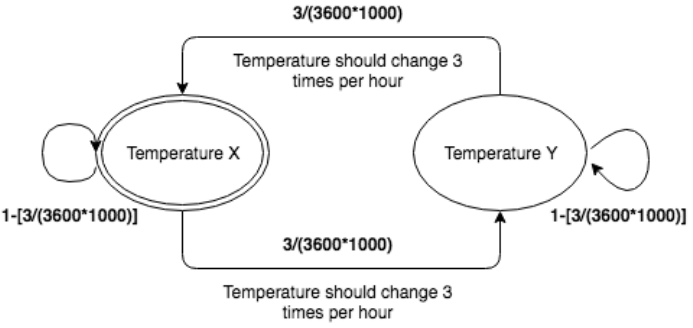
\includegraphics[width=1\linewidth]{temperature-sensor}
        \caption{Temperature Sensor model}
        \label{fig:temperature-sensor}
    \end{subfigure}
    \begin{subfigure}[b]{.5\textwidth}
        \centering
        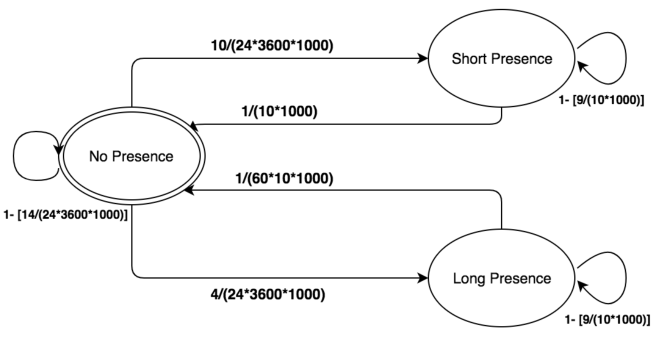
\includegraphics[width=1\linewidth]{presence-sensor}
        \caption{Presence Sensor model}
        \label{fig:presence-sensor}
    \end{subfigure}
    \begin{subfigure}[b]{.5\textwidth}
        \centering
        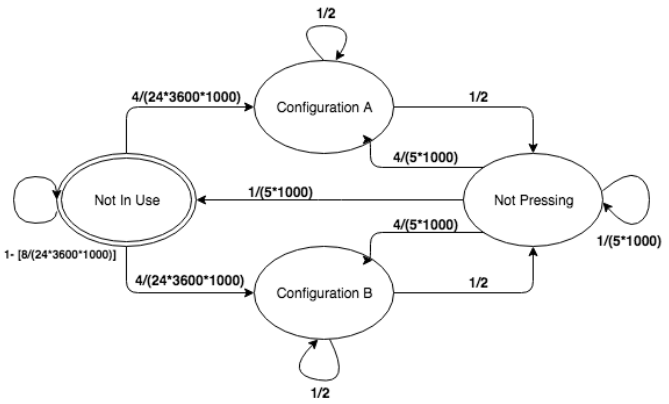
\includegraphics[width=1\linewidth]{tv-remote}
        \caption{TV Remote model}
        \label{fig:tv-remote}
    \end{subfigure}
    \begin{subfigure}[b]{.5\textwidth}
        \centering
        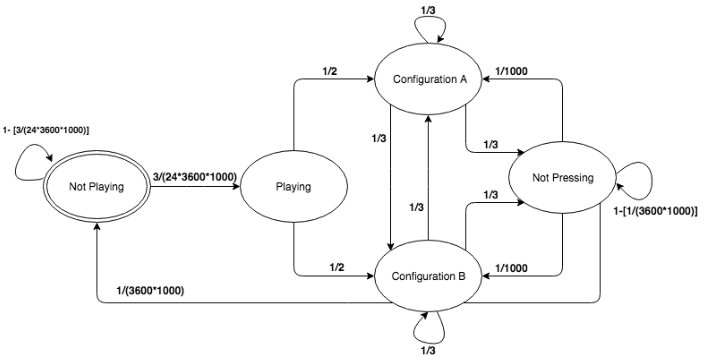
\includegraphics[width=1\linewidth]{joysick-sensor}
        \caption{Joystick model}
        \label{fig:joysick-sensor}
    \end{subfigure}
\end{figure}
\end{centering}\\
Figures \ref{fig:temperature-sensor} to \ref{fig:joysick-sensor}, taken from
\cite{Maselli}, depicts the transition probabilities of the various states a device
could be in. The state change is based on time. Taking fig \ref{fig:temperature-sensor}
for instance, it was found that a temperature sensor produces new data three times in
an hour hence the various probabilities with respect to time in milliseconds.
There are two states in with a temperature sensor and with a probability of 
$3/(3600*1000)$ it changes from, lets say, state X to Y or vice versa and with
$1-3/(3600*1000)$ stays in its state.\\\\
\begin{centering}
\begin{figure}[h!]
    \begin{tikzpicture}
        \tikzumlset{font=\tiny\ttfamily}
        \umlemptyclass[x=-3.5,y=0]{Application}{
        }{}
        \umlclass[x=2.5,y=-2]{SensorNode}{
            -m\_port : uint16\_t \\ -m\_PreState : uint16\_t \\ m\_received :
            uint64\_t \\ -m\_socket : Ptr$\langle$Socket$\rangle$ \\
            -m\_lossCounter : PacketLossCounter
        }{
        +SensorNode() \\
        \umlvirt{$\sim$SensorNode} \\
        \umlvirt{-StartApplication(void) : void} \\
        \umlvirt{-StopApplication(void) : void} \\
        \umlvirt{\#DoDispose(void) : void} \\
        -HandleRead(socket : Ptr{\tiny$\langle$}Socket{\tiny$\rangle$})
        : void \\ -indexOfLargestProb({\tiny\&}matrix : Matrix) : int \\
        -CopyMatrix({\tiny\&}from : Matrix, {\tiny\&}to : Matrix) : void \\
        -MultMatrix({\tiny\&}trsMtx : const Matrix, {\tiny\&}trsMtxb
        : const Matrix) : Matrix \\
        \umlstatic{+GetTypeId(void) : TypeId} \\ +GetLost(void) : const uint32\_t \\
        +GetReceived(void) : uint64\_t
    }
    \umltypedef[x=-1.5,y=-6]{Matrix}{}{}
    \umlemptyclass[x=-3.5,y=-3.5,template={T,U}]{std::vector}{}{
    }
    \umlclass[x=4.0,y=-7.5]{SensorNodeHelper}{
        -m\_factory : ObjectFactory \\
        -m\_server : Ptr{\tiny$\langle$}SensorNode{\tiny$\rangle$}
    }
    {
        +SensorNodeHelper() \\ +SensorNodeHelper(port : uint16\_t) \\
        +SetAttribute(name : std::string , {\tiny\&}value : const AttributeValue) \\
        +Install(c : NodeContainer) : ApplicationContainer \\
        +GetServer(void) : Ptr{\tiny$\langle$}SensorNode{\tiny$\rangle$}
    }
    \umlenum[x=9.5,y=-4.1]{HeaderValidation}
    {
        BROADCAST : uint16\_t \\ BROADCAST\_REPLY : uint16\_t \\ DATA : uint16\_t
        \\ DATA\_REPLY : uint16\_t \\ STATE\_CHANGED : uint16\_t \\
        STATE\_NOT\_CHANGED : uint16\_t
    }{}
    \umldep[geometry=-|]{Matrix}{std::vector}
    \umldep[geometry=-|]{SensorNode}{Matrix}
    \umlinherit[geometry=-|]{SensorNode}{Application}
    \umlaggreg[geometry=-|]{SensorNode}{HeaderValidation}
    \end{tikzpicture}
    \caption{Class Diagram - Sensor Nodes}
    \label{fig:SensorNodes}
\end{figure}
\end{centering}
Markov Chain with a transition probability, say \textbf{$T$}, and an initial state
probability vector distribution \textbf{$q$}. The probability of the chain being in
state $S_i$ after $n$ steps is the $i^{th}$ entry in the vector given by
\begin{equation}
    q^n = q*( T)^n
    \label{eq:markov}
\end{equation}
To simulate the state change based on equation \ref{eq:markov} and also, taking into
account the discrete time with which the changes occur. The next state vector
probability was computed with the $n^{th}$ step being the current time stamp of the
simulation.\\\\
For each tag-augmented sensor node, when a packet is received, the header is checked
to determine the type of packet. If the packet is that of broadcast, a broadcast
reply is automatically sent to the reader with a payload of the current data.
A data request packet require the sensor node to reply with data. A current state
vector probability is calculated and the index with the maximum value is the state 
of the sensor node. If the computed current state is the same as the previous state,
a \textit{state-not-changed} flag is set in the packet header, data reply flag is 
also set and packet sent to the reader.\\\\
The difference in the various sensors is their transition matrix and the initial
state vector, as shown in \ref{fig:temperature-sensor} - \ref{fig:joysick-sensor},
hence the one class for all the sensor nodes.\\\\
Class diagrams of the \textit{SensorNode} class and its \textit{helper} class are
shown in figure \ref{fig:SensorNodes}. A brief explanation regarding the tasks of
the essential functions of the classes follows.
\begin{itemize}
\renewcommand{\labelitemi}{}
\item \textbf{StartApplication:} the first function run to start the application.
    It sets up a socket, binds it to a local address and configures the function
    to handle a received packet.
\item \textbf{StopApplication:} stops the application by resetting the
    packet-received call back function and closing the socket.
\item \textbf{HandleRead:} this is the packet-received call back function. It is
    invoked when a new packet arrives in the socket or when there is data/packet
    to be read in the socket file. The type of packet received is determined by
    examining the header. A broadcast-reply is sent back to the reader if a broadcast
    packet is received by setting the broadcast-reply flag in the header. For a
    data-request packet, the current state of the sensor node is retrieved from the
    \textit{NextState} function and compared with the previous state. If the states
    (previous and current) are equal, data-reply and state-not-changed flags are set
    in the packet header and if the states differ, state-changed and data-reply
    flags are set. The packet is then sent to the reader.
\item \textbf{NextState:} the state of the sensor node is computed by this function
    which takes the current time stamp as a parameter. \textit{Next-State} is found
    by multiplying previous state vector probability with the time-stamp square of
    the transition probability matrix gotten from multiplying the transition matrix
    time-stamp times, hence the need for a matrix multiplication and copy functions.
\end{itemize}
\textit{SensorNodeHelper} class has functions that aid in the installation of sensors
onto nodes; \textit{Install} function, setting the attributes that were declared in
\textit{GetTypeId} function of the \textit{SensorNode} class with \textit{SetAttribute}
which takes the name of the attributes and the value to be set as parameters. There are,
of course, the constructors and a function that return a pointer to the associated
server.

\subsection{Querier}

\begin{centering}
    \begin{figure}[h!]
        \begin{tikzpicture}
            \tikzumlset{font=\tiny\ttfamily}
            \umlemptyclass[x=-4.0,y=1]{Application}
            {}{}
            \umlclass[x=3.0,y=-3.5]{Querier}
            {
                -m\_sendEvent : ns3::EventId \\ -m\_bonus : double \\
                -m\_malus : double \\ -m\_learningRate : double \\
                -m\_nodeAddress : std::vector$\langle${ns3::Address}$\rangle$ \\
                -m\_reward : std::vector$\langle${double}$\rangle$ \\
                -m\_sReward : std::vector$\langle${double}$\rangle$ \\
                -m\_peerPort : uint16\_t \\ -m\_peerAddress : ns3::Address \\
                -m\_socket : Ptr$\langle${Socket}$\rangle$ \\ -m\_sent : uint32\_t
            }
            {
                +Querier() \\
                \umlvirt{$\sim$Querier()} \\
                \umlstatic{+GetTypeId(void) : ns3::TypeId} \\
                +SetRemote(ip : ns3::Address , port : uint16\_t) : void \\
                +SetRemote(ip : ns3::Address) : void \\
                \umlvirt{\#DoDispose(void) : void} \\
                \umlvirt{-StartApplication(void) : void} \\
                \umlvirt{-StopApplication(void) : void} \\
                -Send(void) : void \\
                -HandleRead(socket : Ptr$\langle${ns3::Socket}$\rangle$) : void \\
                -UpdateReward(reward : std::vector$\langle${double}$\rangle$ ,
                bonusORmalus : double , index : int) :
                std::vector$\langle${double}$\rangle$ \\
                -SoftMax(reward : std::vector$\langle${double}$\rangle$)
            }
            \umlenum[x=10,y=-9.3]{HeaderValidation}
            {
                BROADCAST : uint16\_t \\ BROADCAST\_REPLY : uint16\_t \\
                DATA : uint16\_t \\ DATA\_REPLY : uint16\_t \\
                STATE\_CHANGED : uint16\_t \\ STATE\_NOT\_CHANGED : uint16\_t
            }
            {}
            \umlclass[x=1,y=-9.0]{QuerierHelper}
            {
                -m\_factory : ObjectFactory
            }
            {
                +QuerierHelper() \\
                +QuerierHelper(ip : Address) \\
                +QuerierHelper(ip : Address , port : uint16\_t) \\
                +SetAttribute(name : std::string, ${\&}$value : AttributeValue
                                const) \\
                +Install(c : NodeContainer) : ApplicationContainer
            }
            \umlinherit[geometry=-|]{Querier}{Application}
            \umlaggreg[geometry=-|]{Querier}{HeaderValidation}

        \end{tikzpicture}
    \end{figure}
\end{centering}
